\section{Results \& Discussion}
\label{sec:ResAndDisc}


\subsection{Identification of reduction agent}

\myworries{Put up list of reduction agents tried}
\myworries{Add label!!}

NaBH4 has been described in the literature to produce gold nanoparticles in tunable sizes, depending on the ratio between NaBH4- and gold concentration \cite{NaBH4UsedForGoldNP}. To account for the already acidic environment coming from the gold salt itself, we introduced another group, that consisted of a combination of \ce{NaBH4} and \ce{NaOH} by 1:1 ratio, where NaOH as a sodium base, should moderate the reduction to happen in a less acidic environment.
Hydroxylamine as reducing agent is widely known and has already been described in the context of production of silver colloids \cite{Leopold}.  
As proposed by work done by Goia, Kimming and Turkevich, we added Ascorbic Acid (AscAc), Citric Acid (CitrAc) and a reducing sugar (here: Glucose) to the tested reduction agents. \cite{Goia, Kimling, Frens}

There were 3 samples per reduction agent. Following the heuristic approach, where we optimised the knowledge gain per sample-ratio, we subdivided each group by three different reduction agent immersion times, which were 20 minutes, 40 minutes and 2 hours, respectively. This means that every permutation-group [Reduction Agent/Reduction agent Immersion Time] had one sample.

\myworries{AddGraph of $t_{Red}$ v $R_0$}\\
\myworries{Add Label too}

\paragraph{NaBH4}
During Production we followed the standard procedure with the concentration stated. \ce{NaBH4} is known to hydrolyse in solute and therefore, the intended reactivity is reduced. To decrease premature hydrolation, the \ce{NaBH4}-solution was prepared just before usage and put on ice between production and use. Upon immersion of fiber in \ce{NaBH4}, the production of bubbles could be observed as can be seen in figure \ref{unknown-marker} \myworries{Add Label for Bubbly picture in Appendix.}.

The following equation describes the oxidation-half reaction in this sample:

\begin{center}
\schemestart 
\ce{[BH4]-} + \ce{H+} + 3\ce{H2O}   \arrow{->} \ce{H3BO3} + 4\ce{H2{(g)}}, 
\schemestop\par 
\end{center}

With the stated concentration in table \ref{unknown-marker}, we were able to measure conductivity in all three samples as can be seen in figure \ref{unknown-marker}. We acknowledge the fact that one sample is not sufficient for any significant statement. Nevertheless, we see a tendency of a decreasing resistance when increasing the immersion time, exhibiting a time-dependency in this relation. As a general rule, chemical reactions are known to target a certain ratio between reactant and product \myworries{add reference}. This principle could explain the time-dependency. The produced hydrogen gas evades the liquid reaction solution continuously as seen in picture \myworries{addRef for bubbly Picture}. This imbalance between reactant and product is counter-steered by a shift towards the product side present in the solution, which over time would lead to a steady-state, where the increased concentration of \ce{H3BO3} compensates for the lack of \ce{H2{(g)}}. However, as long the reaction did not reach the steady state, gold atoms will be produced and nuclei will grow. Implicitly this includes the decrease in resistance whose end is marked by a critical point that is governed by reaching the ratio described above or the nanoparticle size.

Scanning Electron Microscopy (SEM) pictures showed a largely heterogeneous distribution of nanoparticles. However, EDS analysis of the crosssection of the fiber reveals gold coating. \myworries{Add Ref}

\paragraph{\ce{NaBH4}/\ce{NaOH}}
\myworries{Check if there are lab-pictures. Refer to them. We did not take SEM/EDS pictures}.


\paragraph{Hydroxylamine}
Production was done according to protocol and with the concentration stated. No conductivity was measured. Nevertheless, SEM pictures revealed successful reduction of gold into round nanoparticles that at some location formed large colloids. \myworries{Add Ref for HyA Picture} Following the principle of Occam's razor, we hypothesise that in the process of the reaction, eventually, the nanoparticles grew to big and subsequently "fell off" the fiber. This explains the phenomenon of no conductivity without any particles.


\paragraph{Ascorbic Acid}
Production was done according to protocol and with the concentration stated. The conductivity measured was 25-43 $\Omega$ and outperforms the next best reduction agent by almost 4 orders of magnitude in the described setup. 


\paragraph{Citric Acid}
The citric acid protocol was slightly changed, upon suggestion by work done by Kimling \cite{Kimling} to include an initiating element to facilitate the formation of nuclei, which then - according to explanation found in chapter \ref{subsec:Perc} - should suffice for produced gold atoms to associate to the nucleus and finally nanoparticles to grow. The identified initiators where heat-exposition and UV-irradiation. For each of those two subgroups, only one sample was prepared.

We prepared the heat exposition group following standard procedure up until the immersion of the fiber in the reduction agent (i.e. citric acid in this case). Using the hot plate, we prepared the citric acid solution to be between 100-120 \degree C, before the fiber was immersed. Over the course of 35 minutes the solution changed from faintly blue and turbid to a clear solution with red particles floating in the solution. A picture of the solution after letting it cool down is shown on page \ref{unknown-marker} \myworries{Add Citric Acid Picture}. The described behaviour replicates the description by Frens\cite{Frens}. Yet, we were not able to measure current.

Using a Demetron Optilux 500, we irradiated one sample after immersion  citric acid solution. The picture on page \ref{unknown-marker} \myworries{Add Picture of Bubbly and reference it} shows the emergence of bubbles at the fiber-solution-interface during irradiation. Comparison with a control citric acid group, where bubble formation was absent, leads to conclusion the phenomenon is caused by the irradiation. However, the integrity of the fiber was impaired. Attempts to take it out the petri dish, showed that the polyurethan fiber was thinned out substantially and sticked on the petri dish. Obviously, there was an influence of the UV-light on the fiber. Further experiments with variable irradiation times and/or intensities, could lead to a more thorough explanation. No conductivity measurement was done in this group.


\myworries{Add UV-Fiber Picture}


\paragraph{Glucose}
Upon suggestion by Kimling \cite{Kimling}, we kept the reduction agent solution at around 30 \degree C during the whole immersion time, using the hot plate. After 15 minutes, some of the solution clearly visible condensed on the closing lid of the petri dish \myworries{Add Picture of PetriDish}. We were not able to measure any conductivity in this sample. However, SEM pictures revealed the formation of gold nanoparticles. Upon further magnification, the peculiar structure of those nanoparticles became visible. The nanoparticles had cracks, which in bigger ones would reveal the pitch black cavities. Due to technical difficulties, the SEM in this setup is not able to image those, but it looks like the nanoparticles are hollow, with the apparent nanoparticles being merely a nanoparticle-shell. The cracks can also be seen on the surface of the fiber. Further experiments with variable temperature and heating times maybe can provide more information on the origin of this behaviour.\\

%\hfill \newline

All reduction agents tested effectuated a change in fiber colour when following the described protocol. As indicated in chapter \ref{subsec:GoldSalt}, this shows that in the experimental setup the reduction of gold was successful. If not stated otherwise the sample did not lead to any behaviour that was worth noting, neither when analysing the reduction agent solution after sample immersion or the fiber by eye.

However, due to the fact no reduction agent but \ce{NaBH4} and \ce{AscAc} did lead to conduction in our fibers, we also conclude that the sheer reduction of gold is not enough to functionalise our fiber with conductivity. In order to explain the relation ship between the reduction agents and the conductivity of the fiber, we have to introduce another metric, which we propose to be the quality of the gold nanoparticles.

\myworries{Here SEM/EDS Pictures Pictures}

As can be seen in the SEM pictures \myworries{ref The SEM pictures} we can partially explain the conductivity by uniformity in spatial distribution and size of the nanoparticles. Further experiments could elucidate which of these factors weigh how much into the equation that explains conductivity in our fibers. 

\subsection{Optimisation}
Encouraged by the good results we decided to optimise for AscAc before making baseline resistance tests for new reduction agents. Additionally, we now took not only the baseline resistance into account but also its behaviour when put under strain stress. This measurement reflects now more the true use case and should reduce misdirected optimisation. The five independent variables defined in chapter \ref{subsec:SampleFab} are now reduced to four. If not different stated, following applies: \begin{center}$c_{AscAc}=0.19M$, $t_{AscAc}=20min$, $c_{Gold}=0.25M$ and $t_{Gold}=1h$
\end{center}
Next we assigned each of those independent variables an anticipated effect size. By intuition we assigned them in the following order, where $>$ marks "has the bigger anticipated effect size than":

\begin{equation}
    c_{AscAc} > c_{Gold} > t_{AscAc} > t_{Gold}
\end{equation}

\subsubsection{Variation of Gold Concentration}

Gold concentration was varied to be $0.025M, 0.25M$  and $0.6M$, respectively.

\begin{figure}[H]
    \centerline{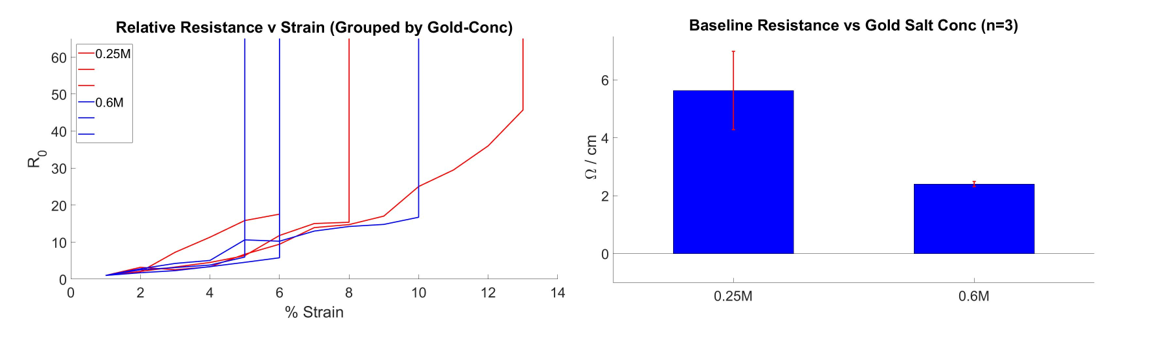
\includegraphics[scale=0.7]{./pic/R0vGoldConc.PNG}}
    \caption{Variation of Gold Concentration}
    \label{fig:GoldConc}
\end{figure}

The $0.025M$-samples did not lead to measurable conduction. The result of the baseline resistance seemingly favours a higher gold concentration. However, the data of strain resistance does not allow for a similarly clear statement, neither when plotting the absolute resistance nor when plotting the normalised one, as we see in figure \ref{fig:GoldConc}, left. The sudden peak out of the plotted range mark the critical point, where conductivity in the fiber was lost and no current was measured. Relaxation of strain also led to regain of measurable conductivity similar to a priori values (not shown).

\subsubsection{Variation of Reduction Agent}


\begin{figure}[H]
    \centerline{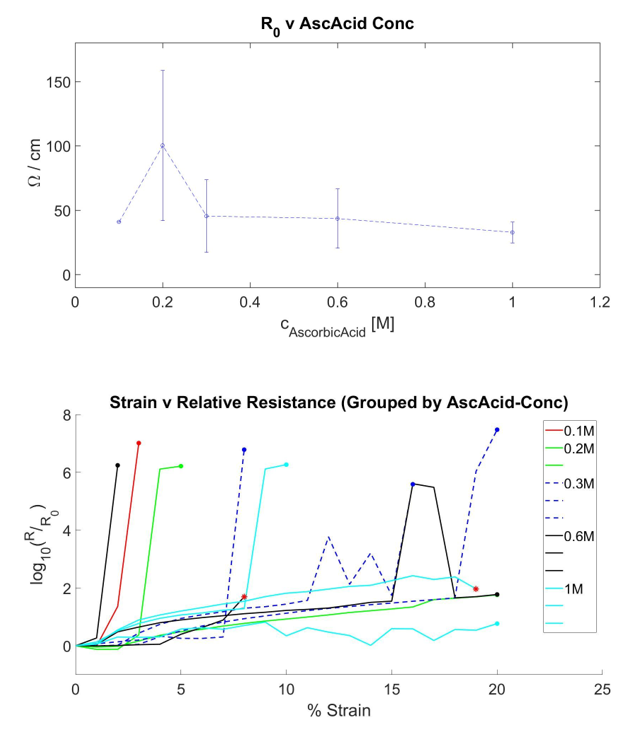
\includegraphics[scale=0.7]{./pic/StrainVAscAcidConc.PNG}}
    \caption{Variation of Gold Concentration}
    \label{fig:GoldConc}
\end{figure}
